\chapter{Preliminary and Future Work}\label{chap:chap3}

\section{Preliminary Work}

In the initial step of work, we superficially explored ChatGPT's ability to generate tests for an example conflict of Point, where a distance method is altered from euclidean to manhattan in one branch and in the other branch, a move method is changed from using the value 1 for x and y movement to using the result of the distance calculation.

We tested two frameworks, first just asking for a test, with prompts based on the testing indications given by the DSL for the case:

\begin{itemize}
  \item A Dependency Based semantic conflict was possibly introduced in a 3-way merge. Develop a test for the class Point, that covers the methods move() and distance(), without calling distance() directly.
Before the merge, the class under test was: [base Point]
After the merge, it was: [merged Point].
  \item A Dependency Based semantic conflict was possibly introduced in a 3-way merge. Develop a test for the class Point, that covers the methods move() and distance(), without calling distance() directly.
Before the merge, the class under test was: [base Point]
In the branch A it was changed to: [A Point]
In the branch B it was changed to: [B Point]
After the merge, it was: [merged Point].

\end{itemize}

For this, the LLM simply took one version and created tests taking it as correct behaviour. In the first case, for Base and in the second for Merge. This is not ideal, as the first does not allow us to distinguish if the behaviour changed due to merging, or just do to changes in the branches. The latter takes merge as correct behaviour and will thus always fail.

Other tests involved first asking for an explanation if there was a merge conflict there, before asking for a test

\begin{itemize}
  \item We have done a merge on a piece of code.
Before the merge, the code was: [code]

In the branch A it was changed to: [code]

In the branch B it was changed to: [code]

After the merge it was: [code]

Do you believe there could be a merge conflict here? Where? Explain why.
  \item We have done a merge on a piece of code.
  
Before the merge, the code was: [code]

In the branch A it was changed to: [code]

In the branch B it was changed to: [code]

After the merge it was: [code]

Do you believe there could be a merge conflict here? Where? Explain why. Pay attention to both additions and modifications.
  \item We have done a merge on a piece of code code.
  
Before the merge, the code was: [code]

In the branch A it was changed to: [code]

In the branch B it was changed to: [code]

After the merge it was: [code]

Do you believe there could be a *semantic* merge conflict here? Where? Explain why. Pay attention to both additions and modifications.

\end{itemize}

The first two prompts failed. Indeed for prompt ChatGPT only mentioned the changes in move, but even after prompting it to pay attention to distance, it failed to identify the conflict. For both, it seemed to not understand what was being referred to when speaking of conflict, describing all changes as a "conflict". Thus it would say, there is a conflict between whether to use euclidian and manhattan distance and there is a conflict on how the move function works.

The last prompt given, highlighting the *semantic* aspect of the merge conflict, yielded good results, with the conflict being perfectly described, as seen in figure \ref{fig:semconf}. After prompting for a test, it generates an appropriate one: it tests if the move function updates Point appropriately based on the euclidean distance. Thus it fails for base and branch B, where movement is still done with the value of 1, it passes for branch A as there move is based on distance; and it fails in merge, as now movement is being done with the distance calculation, but the calculation is now manhattan.

\begin{figure}
    \centering
    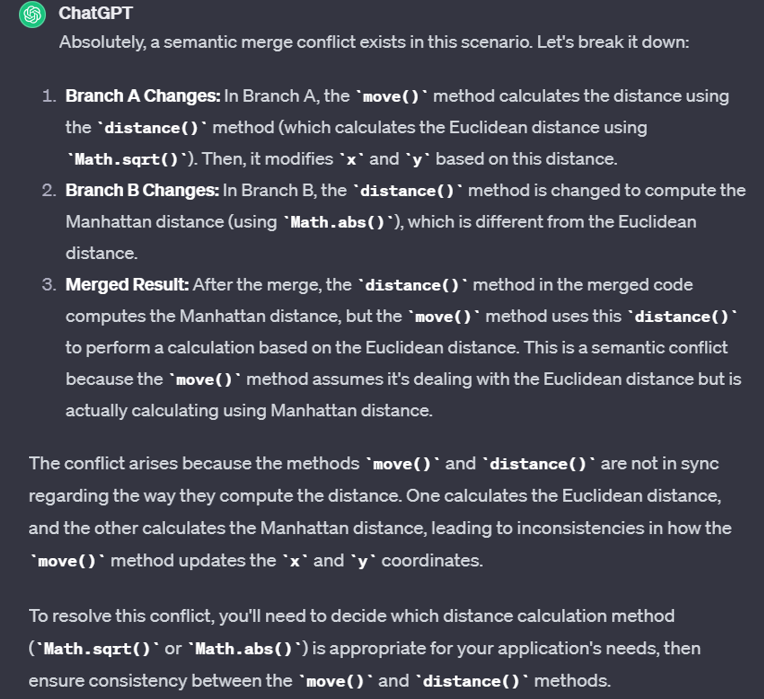
\includegraphics[width=0.75\linewidth]{figures/image.png}
    \caption{ChatGPT description of the semantic conflict}
    \label{fig:semconf}
\end{figure}

In simple fabricated scenarios, where simple conflicts were added to existing software solutions, ChatGPT showed ability to identify and describe the semantic conflict. Despite this, test generation remained complicated and few of the successful identification of semantic conflicts yielded working tests. The final prompt follows.

\begin{quote}
Generate a Junit unit test to identify this semantic conflict, knowing what you do now. The test must compile without errors and require no further alterations. It should require no further dependencies and import all classes correctly.
\end{quote}

While adapted to avoid common pitfalls, the tests generate still suffered from basic issues such as missing imports, which can be mitigated by prompting the LLM for correction automatically. More complex issues of implementation, such as calling the base function instead of dependent, wrong usage of construction and function returns, parameter types or unnecessary mocks. Further, when prompting for correction, the LLM often explains that the developer should correct this, thus further work needs to be done to ensure the tool does all the work itself.

Prompting in real-world examples, or more complex fabricated examples, has produced far worse results. Several refinements were made to the prompts, most significantly: the usage of "git diff" to highlight the specific changes in branch A and branch B, the explanation of the conflict present and the specification of the target method where the conflict is evident. These modifications were largely unsuccessful and did not lead to identification of any conflicts.

We also had to reckon with size limits for messages. Thus, we started with an explanatory prompt and then feed the information step by step. However, it remained crucial to remind the LLM of the goal in the last message.

\begin{quote}
We have done a merge on a piece of software and introduced a semantic conflict of types: "Update two different dependencies of a method or update one method and concurrently update one of its dependencies" and "Concurrent changes to the same method". I will now show the base commit, the diff in branch A, the diff in branch B, and the final merge version in 4 separate messages. At the end I want you to explain why and where the semantic conflict is present.
\end{quote}

Common issues are confusion between textual and semantic merges, which can be mitigated by clear explanation of what a semantic merge is; hallucinations of features not present in the code or hallucinations of changes where changes were not made; lack of focus on the methods where conflict is evident, despite reiterations; loss of focus when prompt has to be split into several messages. When the tools do understand the semantic conflict, the best description they can give is to point out the changes made between branches followed by the suggestion that there may be a conflict there.
Part of the difference between real-world examples and fabricated scenarios may come down to the information given. The fabricated scenarios, based on work of Nuno Castanho \cite{kn:nuno}, were accompanied with a description of the specific semantic conflict present. Thus it is possible collecting and offering that information with real-world scenarios may improve the ability of LLMs in this regard.

Another factor in consideration is the issue of dependencies, as so far testing had focused on just a unitary class. Given that semantic conflicts can involve interactions between classes and subclasses or other dependencies, it is relevant to provide further information. Initial tests just added one dependency, wether by calling a class methods or due to a inheritance relationship. An example, with the addition of an illustrative example of a semantic conflict follows.

\begin{quote}
We have done a merge on a piece of software and introduced a semantic conflict of type Parallel Changes in Method.

Semantic conflicts occur when concurrent and syntactic-correct changes in different regions of a source file or different files cause the software system to misbehave. For example, suppose there is a Java class `Point` with a method `distance()` that computes the Euclidean distance of a Point to the origin and Bob decides to modify `distance()` so it computes instead the Manhattan distance. At the same time, Alice, not aware of Bob's changes, creates a new method `move()` that uses `distance()` to calculate the Euclidean distance. Then, the changes of both developers are merged. As Bob and Alice did not modify the same lines of code, there is no textual conflict. There is neither a syntactic conflict as the merged code still compiles. However, the program now has an unexpected behaviour. The `move()` method introduced by Alice no longer moves a Point an Euclidean distance (as Alice was expecting) but rather moves a Manhattan distance

The affected declaration is copyWithDefaults().

A first message will detail the class before the merge, the diffs for both branches and the class after the merge. A second message will have a dependent class, whose methods indirectly call copyWithDefaults(). After I send these next two classes, identify and describe the semantic conflict.    
\end{quote}

A more complex evolution on this idea consisted of providing textual representations of UML graphs, such as plantUML structure graphs. These however proved to be complex in their own regard as they often induced the LLM to "forget" previous information and its' goal, possibly due to their large size.

No successful tests have been generated for real world scenarios.
Experiments with other LLMs, such as Bing AI or Bard, yield similar problems and new ones, such as more stringent size limits, suggesting an altered approach may have to be taken.



\section{Future Work}

\subsection{Development Plan and Tool Functioning}

Development of the solution will go through several stages. Firstly, the process which has already been in progress, is the initial evaluation of LLM's and prompt techniques. After acquiring the list of subjects to test and deciding on the LLM, we can systematize this to develop the prototype solution. From here we start developing a tool that can automatically generate a prompt, get a test from the LLM and then run it. This prototype tool can then be further augmented, by applying corrections for tests that may fail to compile. Figure \ref{fig:tool} details the expected functioning of the tool once completed. A final period of evaluation and observations will compare our results to previous work and reflect on possible further improvements.

\begin{figure}
    \centering
    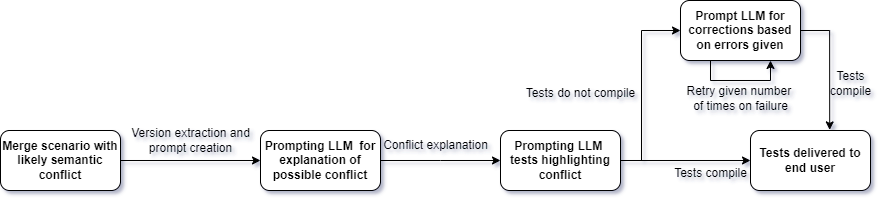
\includegraphics[width=1\linewidth]{figures/tool.png}
    \caption{Functioning pipeline of proposed tool}
    \label{fig:tool}
\end{figure}

\begin{figure}
    \centering
    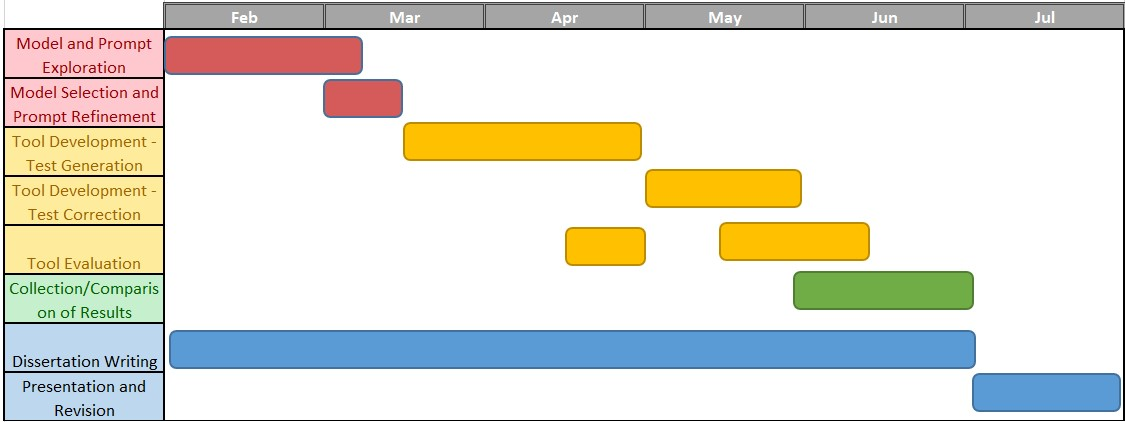
\includegraphics[width=1\linewidth]{figures/gantt.jpg}
    \caption{Gantt diagram of working plan}
    \label{fig:gantt}
\end{figure}

\subsection{Subjects}

To assess the validity of a developed solution, a collection of subjects to test must be collected. While several previous work has compiled collections of merge commits with semantic conflicts, the collection done by Nuno Castanho \cite{kn:nuno} is particularly useful, being publicly available, closely related to our own work, and also allowing us to draw direct comparisons. Most importantly, it aggregates merge instances from both Silva et al \cite{kn:leuson} and Sousa et al \cite{kn:safemerge}, thus being more extensive.

\subsection{LLM's}

While preliminary work sought to explore ChatGPT and Llama (both CodeLlama and Llama 2), hardware constraints meant we were unable to explore Llama. ChatGPT, being hosted online for free, did not suffer from such issues, but future problems may arise, most notably the possibility of the size limit for messages interfering in our work. Going forward we will further explore how to mitigate these and possible alternatives.